\section{Results}
\label{sec:results}

\subsection{Full-training-data comparison}
\label{sec:results-full}

% AUTO-GENERATED by scripts/generate_numbers.py -- DO NOT EDIT BY HAND.
\begin{table}[htbp]
\centering
\caption{Full-training-data (N=full, 4180 cases) comparison. CRPS, twCRPS, and interval width in Kelvin; coverage against the 80\%-nominal p10--p90 band. DRN is trained under a feature-constrained setup (Section~\ref{sec:limitations}), not its originally-intended full feature set.}
\label{tab:full-comparison}
\setlength{\tabcolsep}{4pt}
\begin{tabular}{lcccc}
\toprule
Method & \shortstack{CRPS\\(K)} & \shortstack{twCRPS\\(K)} & \shortstack{Coverage\\@80\%} & \shortstack{Interval\\width (K)} \\
\midrule
Raw ensemble & 1.3590 & 1.1109 & 0.4259 & 2.3716 \\
Var.-inflated, CRPS-optimal (a) & 1.3005 & 0.9522 & 0.7388 & 5.2037 \\
Var.-inflated, fixed $\lambda=1.5$ (b) & 1.3042 & 0.9776 & 0.6096 & 3.7258 \\
Var.-inflated, coverage-matched (c) & 1.3361 & 1.0029 & 0.8221 & 6.7224 \\
Var.-inflated, leakage-optimistic (d)$^{\dagger}$ & 1.3054 & 0.9579 & 0.7603 & 5.5344 \\
TimesFM-3 (zero-shot) & 1.3592 & 1.0268 & 0.7603 & 5.1379 \\
TimesFM-3, two-covariate (mean + spread)$^{\ddagger}$ & 1.3837 & -- & 0.8027 & 5.8246 \\
EMOS pooled & 1.2612 & 0.9138 & 0.8303 & 5.4559 \\
EMOS local & 1.1023 & 0.8239 & 0.8289 & 4.7548 \\
DRN & 1.2251 & 0.8989 & 0.7720 & 4.6494 \\
\bottomrule
\end{tabular}
\par\smallskip
{\small $^{\dagger}$Never a legitimate baseline: $\lambda$ is fit directly on test-set coverage (Section~\ref{sec:methods-list}), an upper bound on what any trivial rescaling could achieve at this coverage target, not a leakage-free result.}\\
{\small $^{\ddagger}$Not this paper's main TimesFM-3 configuration (that is the zero-shot row above, used everywhere else in this paper): an additional experiment supplying ensemble spread as a second covariate (Section~\ref{sec:discussion-covariate-check}). twCRPS is omitted (--) because per-instance quantiles for this run were not persisted; only the aggregate metrics shown were saved.}
\end{table}


At full training data (Table~\ref{tab:full-comparison}), every trained
method beats TimesFM-3 on CRPS: EMOS pooled (\CrpsEmosPooledFull{} K),
EMOS local (\CrpsEmosLocalFull{} K), and DRN (\CrpsDrnFull{} K), against
TimesFM-3's \CrpsTsfmFull{} K and the raw ensemble's \CrpsRawFull{} K.
The trivial variance-inflation baseline beats TimesFM-3 on CRPS too: both
the CRPS-optimal variant (a, \CrpsInflAFull{} K) and the
fixed-climatological variant (b, \CrpsInflBFull{} K) undercut TimesFM-3's
\CrpsTsfmFull{} K, and (b) needs no training data at all -- a single
zero-shot scalar rescaling of the raw ensemble's spread already beats a
frozen foundation model on this metric. On the calibration-sharpness axis
the same trivial rescaling does not match TimesFM-3: the coverage-matched
variant (c), calibrated on training data alone to reach as closely as a
training-fit multiplier allows TimesFM-3's own test coverage
(\CoverageInflCFull{} achieved against a \CoverageTsfmFull{} target,
Section~\ref{sec:methods}), needs \WidthInflCFull{} K to do so --
substantially wider than TimesFM-3's \WidthTsfmFull{} K, even after
accounting for (c) landing closer to the nominal 0.80 target than
TimesFM-3 itself, which alone would call for a somewhat wider interval.
Variant (d), never a legitimate baseline (Section~\ref{sec:methods-list}),
bounds how much of that width gap could be a leakage artifact of (c)'s
train/test split rather than a real limit: fit directly on test-set
coverage, it reaches \InflLeakyCrps{} K on CRPS and
\InflLeakyCoverage{} achieved against the identical \CoverageTsfmFull{}
target -- matched exactly, not merely approximately -- yet still needs
\InflLeakyWidth{} K, wider than TimesFM-3's \WidthTsfmFull{} K even at
this leakage-optimistic upper bound. This margin is not just a point
estimate: a day-blocked bootstrap on the per-instance width difference
gives \InflLeakyWidthDiffPoint{} K (95\% CI
[\InflLeakyWidthDiffCiLow{}, \InflLeakyWidthDiffCiHigh{}]), entirely
positive -- the leakage-optimistic variant is significantly wider than
TimesFM-3, not merely wider on average. The bootstrap resamples
day-blocks around a single leaky multiplier fit once on the full matched
test set; the interval is conditional on that multiplier and quantifies
sampling variability in the width difference, not variability in the
multiplier itself. TimesFM-3's real advantage over
one-parameter rescaling is therefore narrower than a CRPS-only reading
suggests, and it sits on a different axis than CRPS: on CRPS, a trivial
multiplier already beats it, zero-shot; the width/coverage trade-off is
where TimesFM-3 holds an edge that neither a leakage-free nor a
leakage-optimistic scalar rescaling reproduces. Section~\ref{sec:discussion}
returns to what this split result means for claims that trivial baselines
match foundation models generally \citep{zhang_2025_context_parroting}.

A separate experiment supplies TimesFM-3 with ensemble spread as a
second, simultaneous covariate (Table~\ref{tab:full-comparison}'s
two-covariate row). CRPS worsens to \CrpsTsfmTwoCov{} K and coverage
moves closer to the 0.80-nominal target (\CoverageTsfmTwoCov{} against
\CoverageTsfmFull{}) at a substantially wider interval
(\WidthTsfmTwoCov{} K) -- a shift along the calibration-sharpness
trade-off, not a clean improvement, discussed fully in
Section~\ref{sec:discussion-covariate-check}.

\subsection{The training-data-size breakpoint curve}
\label{sec:results-breakpoint}

\begin{figure}[htbp]
\centering
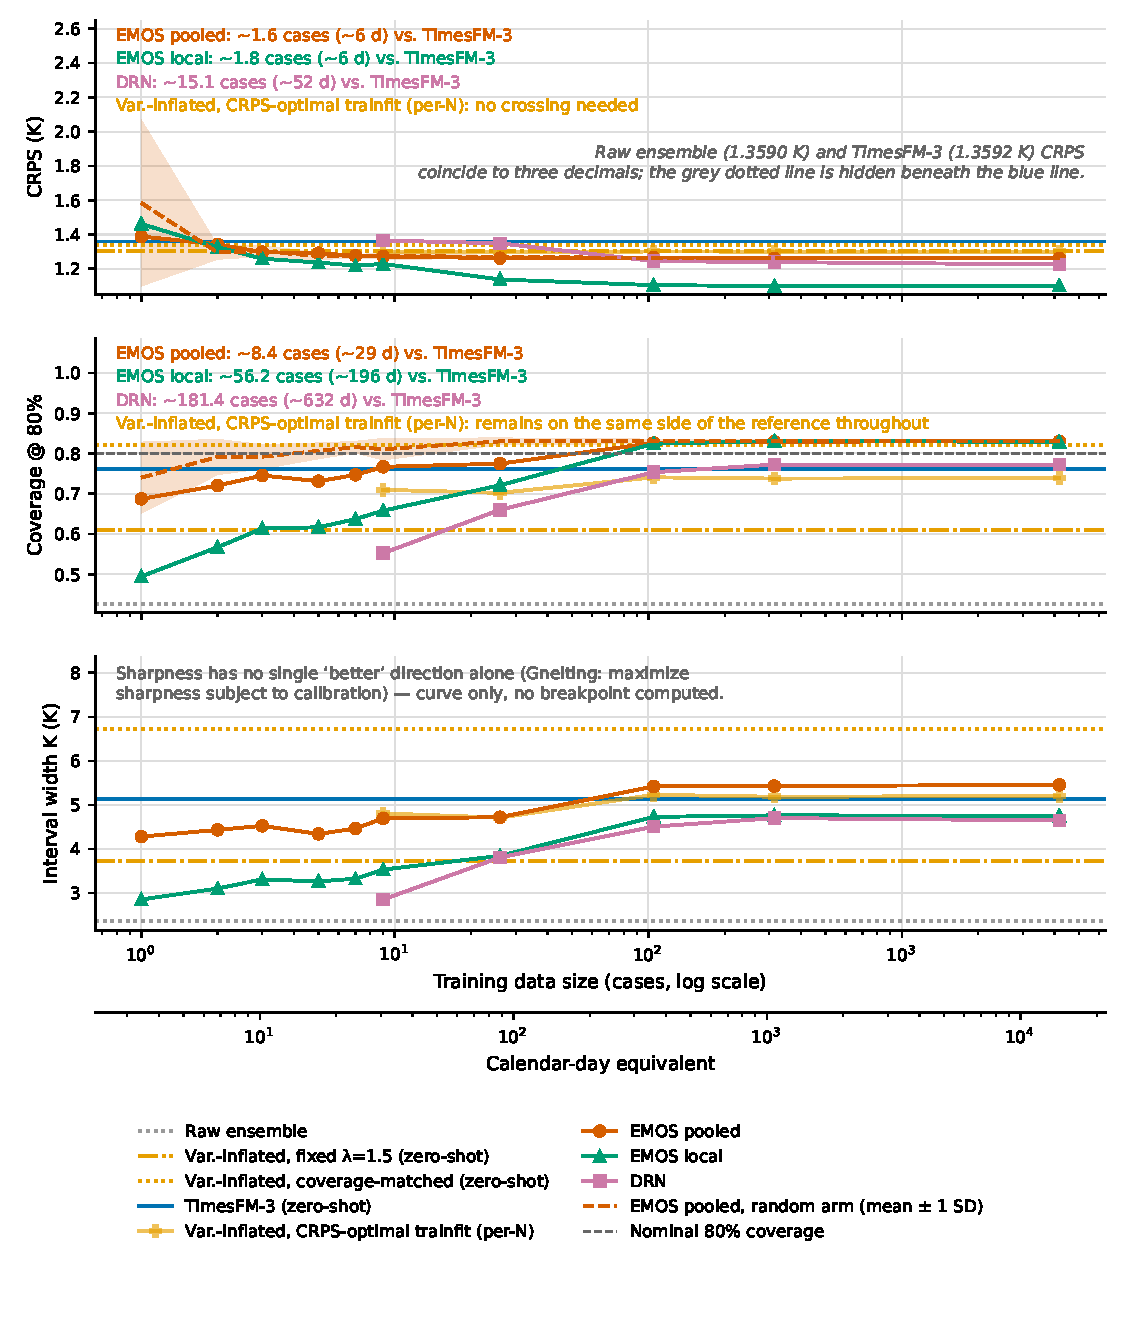
\includegraphics[width=0.95\linewidth]{figures/f1_breakpoint_curve}
\caption{CRPS, coverage@80\%, and interval width against training data
size (cases, log scale, with calendar-day equivalent on the secondary
axis). Horizontal lines are N-independent zero-shot references; curves are
trained methods refit at each N.}
\label{fig:f1}
\end{figure}

Figure~\ref{fig:f1} shows the paper's headline result: EMOS crosses
TimesFM-3's CRPS at \BpCrpsPooledCases{} cases pooled
(\BpCrpsPooledDays{} calendar days) and \BpCrpsLocalCases{} cases locally
(\BpCrpsLocalDays{} days). That raw crossing is a point estimate, not
itself statistically significant: testing significance at every
low-\(N\) point on this curve (\(k=1,2,3,5,7,9\), Section~\ref{sec:results-significance})
shows the advantage is significant from \BpCrpsPooledSigK{} cases
(\BpCrpsPooledSigDays{} calendar days) onward for pooled EMOS and from
\BpCrpsLocalSigK{} cases (\BpCrpsLocalSigDays{} days) for local EMOS --
under day-blocking, our primary block definition; the station-blocked
\(t\)-test does not reach significance anywhere in the tested
\(k=1\)--9 range for either variant, while the station-blocked Wilcoxon
test does, from \(k=\BpCrpsPooledStationWilcoxonFirstSigK{}\) onward --
the same test-statistic divergence already reported at \SigTestNCases{}
cases (Section~\ref{sec:results-significance}), now shown to persist
across the whole low-\(k\) range. Both numbers matter and neither
replaces the other: the raw crossing (\BpCrpsPooledDays{} days) is where
the two methods' CRPS point estimates change order; the day-blocked
significant crossing (\BpCrpsPooledSigDays{} days) is where that
difference is established rather than plausibly noise. DRN needs
\BpCrpsDrnCases{} cases (\BpCrpsDrnDays{} days) -- under the
feature-constrained setup this paper trains it in, not DRN's
originally-intended full feature set (Section~\ref{sec:limitations}).
The variance-inflation
baseline (variant a, CRPS-optimal, refit per training size the same way
EMOS is) is already better at the smallest tested N: at
\InflASmallestNDays{} days it already reaches \InflASmallestNCrps{} K,
below TimesFM-3's \CrpsTsfmFull{} K, and stays there throughout the
tested range -- the same qualitative pattern Table~\ref{tab:full-comparison}
shows at full data (Section~\ref{sec:results-full}). Coverage tells a
different story (ratios below computed from the unrounded breakpoint
estimates, not the values as displayed): EMOS pooled crosses TimesFM-3's
coverage at \BpCoveragePooledCases{} cases (\BpCoveragePooledDays{} days)
-- \CoverageCrpsRatioPooled{}x later than its CRPS crossing -- and EMOS
local not until \BpCoverageLocalCases{} cases (\BpCoverageLocalDays{}
days), \CoverageCrpsRatioLocal{}x later than its own CRPS crossing; DRN crosses
at \BpCoverageDrnCases{} cases (\BpCoverageDrnDays{} days). Interval width
has no crossing at all (Section~\ref{sec:breakpoint-def}): EMOS pooled's interval
starts narrower than TimesFM-3's and crosses to wider somewhere between
90 and 365 training days, while EMOS local stays narrower than TimesFM-3
across the entire tested range even as it reaches comparable coverage --
a sharpness advantage a pooled fit does not share.

\subsection{Lead-time resolution}
\label{sec:results-leadtime}

\begin{figure}[htbp]
\centering
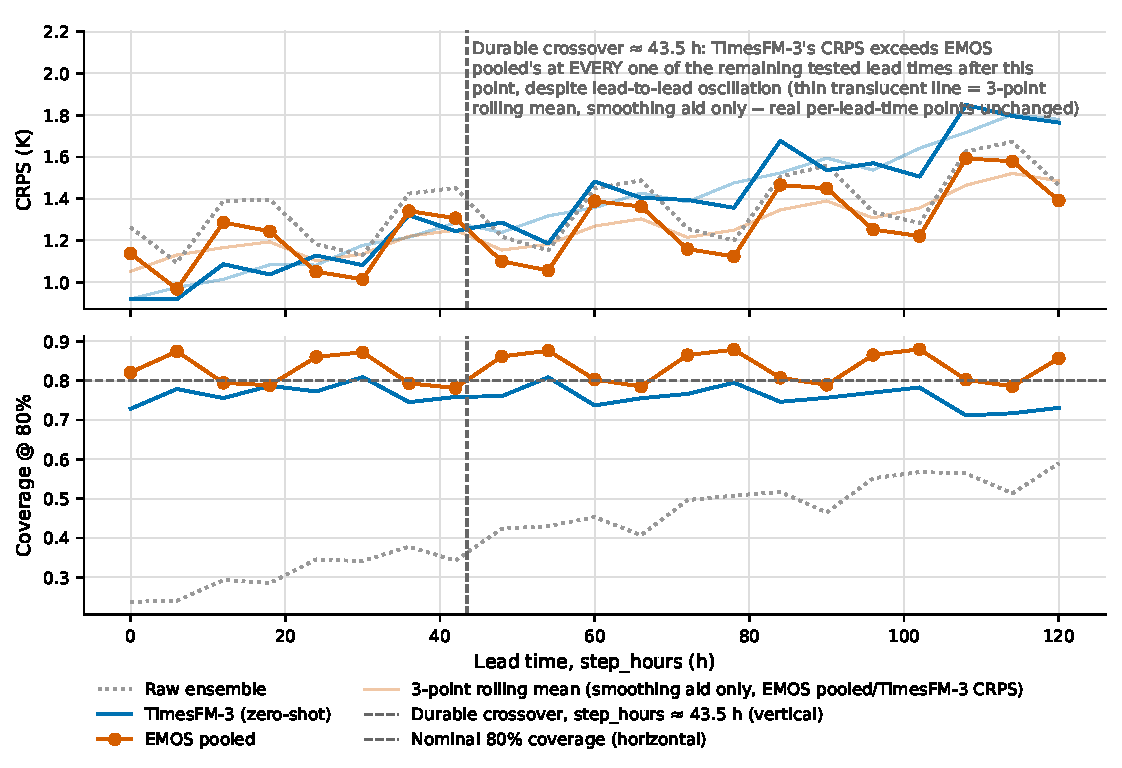
\includegraphics[width=0.95\linewidth]{figures/f2_lead_time_resolved}
\caption{CRPS and coverage@80\% by lead time (21 steps, 0--120~h).}
\label{fig:f2}
\end{figure}

\begin{figure}[htbp]
\centering
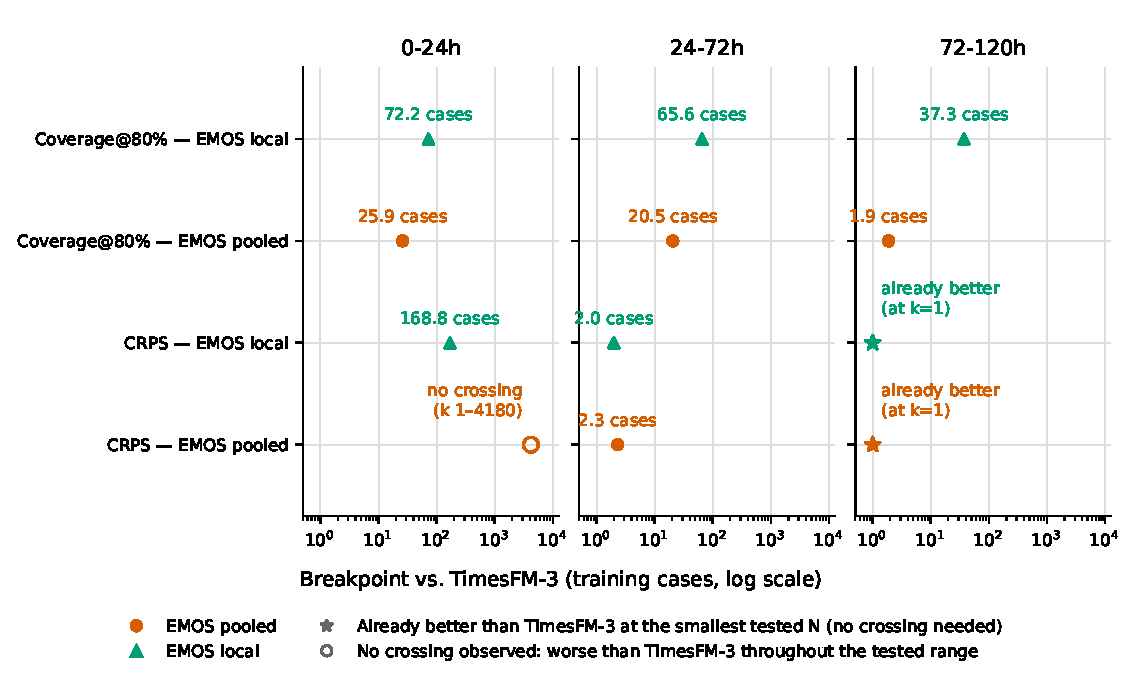
\includegraphics[width=0.95\linewidth]{figures/f5_breakpoint_by_lead_group}
\caption{Training-data-size breakpoint, computed separately within each
lead-time bucket, for CRPS and coverage@80\%.}
\label{fig:f5}
\end{figure}

Pooling over all 21 lead times hides a reversal (Figure~\ref{fig:f2}):
TimesFM-3's CRPS advantage is real but short-lived, with a first sign flip
at \FirstSignFlipHours{}~h and a durable crossover at
\DurableCrossoverHours{}~h, after which TimesFM-3 remains the worse method
at every longer tested lead time. Recomputing the breakpoint curve
separately within three lead-time buckets (0--24~h, 24--72~h, 72--120~h;
Figure~\ref{fig:f5}) sharpens this into the paper's most lead-dependent
result: at 72--120~h, both EMOS pooled and EMOS local already beat
TimesFM-3 on CRPS at the smallest tested training size (a single case);
at 0--24~h, pooled EMOS does not cross TimesFM-3's CRPS anywhere in the
tested range, from 1 to 4180 cases. Coverage crossings follow the same
ordering (earliest at long lead, latest at short lead) but at
substantially larger training sizes than CRPS in every bucket.

\subsection{Sharpness, calibration, and PIT diagnostics}
\label{sec:results-sharpness}

\begin{figure}[htbp]
\centering
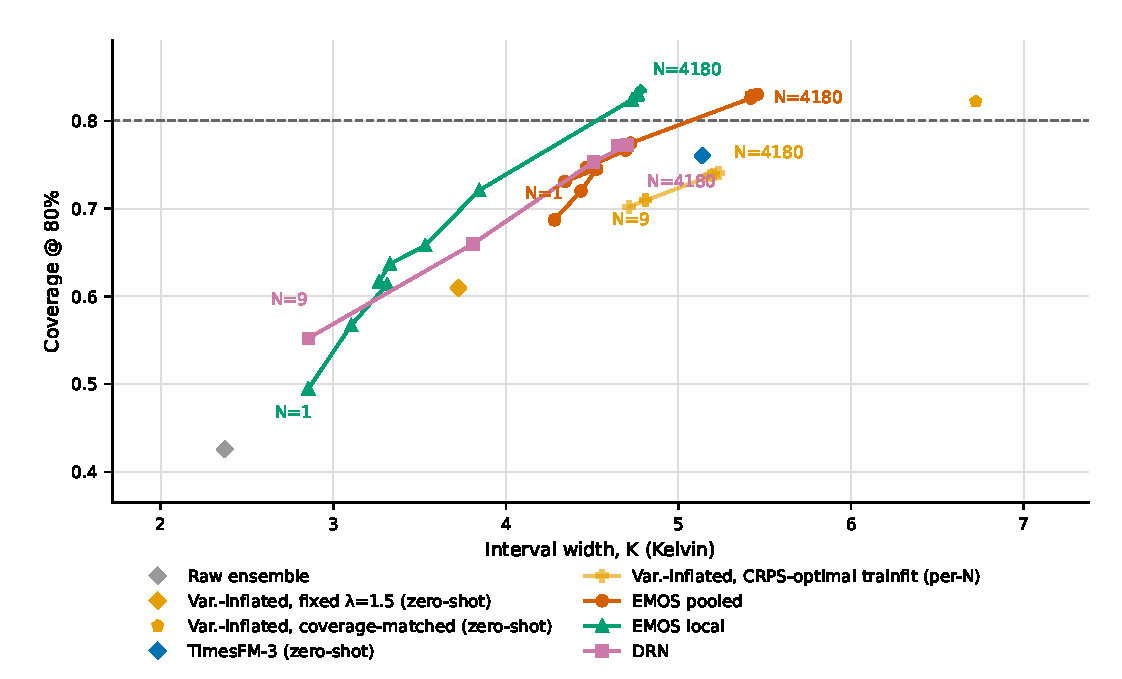
\includegraphics[width=0.7\linewidth]{figures/f3_sharpness_calibration_plane}
\caption{Interval width against coverage@80\% for every method; trained
methods shown as trajectories across training size, zero-shot methods as
single points.}
\label{fig:f3}
\end{figure}

\begin{figure}[htbp]
\centering
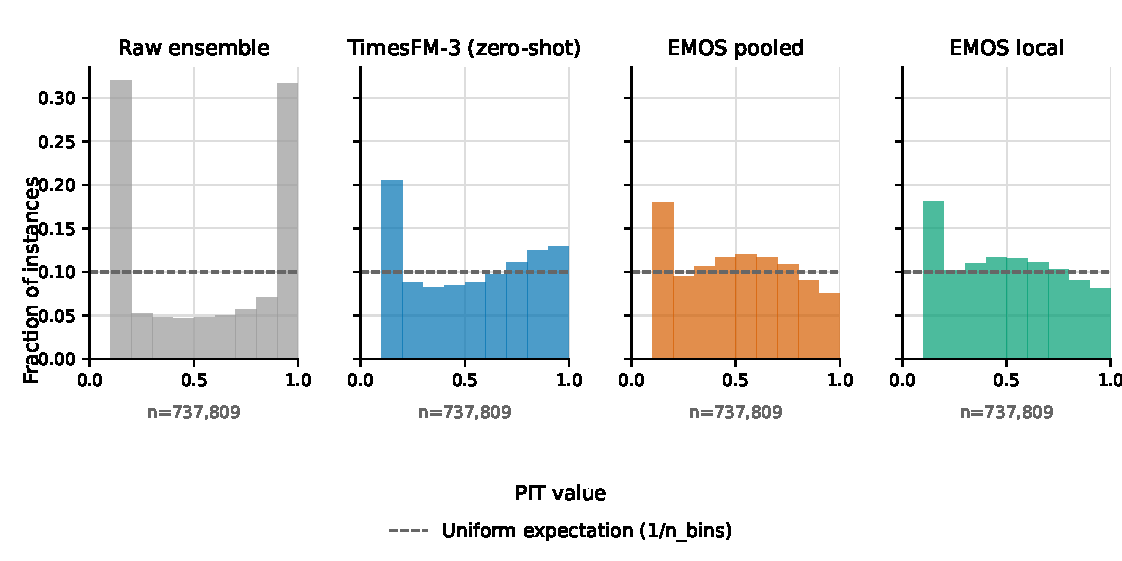
\includegraphics[width=0.95\linewidth]{figures/f4_pit_histograms}
\caption{PIT histograms at full training data. PIT uniformity is assessed
descriptively; no formal uniformity test valid under serial dependence is
applied.}
\label{fig:f4}
\end{figure}

Figure~\ref{fig:f3} makes Section~\ref{sec:results-full}'s width/coverage
trade-off visible directly: EMOS local's trajectory sits up and to the
left of every other trained method's, reaching comparable coverage to
TimesFM-3 with a narrower interval throughout. The raw ensemble's PIT
histogram (Figure~\ref{fig:f4}) shows the classic severe-underdispersion
signature -- roughly a third of observations fall in each of the two
outermost bins -- consistent with its \CoverageRawFull{} empirical
coverage against a 0.80 nominal target; TimesFM-3 and both EMOS variants
show comparatively flat histograms, read descriptively per
Section~\ref{sec:methods}.

Table~\ref{tab:full-comparison}'s twCRPS column follows the same ranking
as CRPS itself for every method (e.g.\ EMOS local's
\TwcrpsEmosLocalFull{} K remains the lowest, TimesFM-3's
\TwcrpsTsfmFull{} K remains among the highest) -- this checks the upper
end of the quantile grid this study fixed for every method, not whether
TimesFM-3 genuinely lacks tail behavior beyond p90
(Section~\ref{sec:metrics}).

\subsection{Statistical significance}
\label{sec:results-significance}

At the pooled headline comparison (EMOS pooled vs.\ TimesFM-3 at
\SigTestNCases{} cases, \SigTestNDays{} days), the CRPS advantage is robust to block
definition: station-blocked and day-blocked tests agree in direction, and
the day-blocked test -- which additionally absorbs cross-station synoptic
dependence the station block cannot -- gives \(p=\SigCrpsDayT\) (paired
\(t\)) and \(p=\SigCrpsDayW\) (Wilcoxon), both far below the station-blocked
test's already-significant Wilcoxon result (\(p=\SigCrpsStationW\)) and its
non-significant \(t\)-test (\(p=\SigCrpsStationT\)). The coverage advantage
does not clear the same bar: station-blocked (\(t\): \(p=\SigCoverageStationT\);
Wilcoxon: \(p=\SigCoverageStationW\)) and day-blocked
(\(t\): \(p=\SigCoverageDayT\); Wilcoxon: \(p=\SigCoverageDayW\)) tests
disagree with each other on both significance and, at the day block,
direction of evidence between the two test statistics. We do not report
EMOS as coverage-superior to TimesFM-3 at this training size: the honest
summary is that the CRPS result is significant under every tested block
definition and test statistic, while the coverage result is not.

The breakpoint curve's own raw crossing (Section~\ref{sec:results-breakpoint}:
\BpCrpsPooledCases{} cases pooled, \BpCrpsLocalCases{} cases locally) is a
different, smaller training size than \SigTestNCases{} cases, and was not
itself significance-tested until now. Repeating the day- and
station-blocked tests at every point on the low-\(N\) breakpoint grid
(\(k=1,2,3,5,7,9\)) shows the CRPS advantage is not significant at the
raw crossing: the earliest \(k\) at which both the day-blocked \(t\)-test
and Wilcoxon test (day-blocking is our primary block definition) agree
the advantage is significant is
\BpCrpsPooledSigK{} cases (\BpCrpsPooledSigDays{} days) for pooled EMOS
(day-blocked \(t\): \(p=\BpCrpsPooledSigKDayT\); Wilcoxon:
\(p=\BpCrpsPooledSigKDayW\)) and \BpCrpsLocalSigK{} cases
(\BpCrpsLocalSigDays{} days) for local EMOS (day-blocked \(t\):
\(p=\BpCrpsLocalSigKDayT\); Wilcoxon: \(p=\BpCrpsLocalSigKDayW\)) --
meaningfully later than the raw crossing, though still a small absolute
training size. The station-blocked paired \(t\)-test is not significant
at this same \(k\) for either variant (pooled: \(p=\BpCrpsPooledSigKStationT\);
local: \(p=\BpCrpsLocalSigKStationT\)), while the station-blocked Wilcoxon
test is (pooled: \(p=\BpCrpsPooledSigKStationW\); local:
\(p=\BpCrpsLocalSigKStationW\)) -- the same station-block
\(t\)-vs-Wilcoxon divergence already seen at \SigTestNCases{} cases above
holds throughout the tested range, not just at that one point; the
station-blocked \(t\)-test is not significant at any \(k\) we tested from
1 to 9 cases for either EMOS variant.

Repeating both block definitions separately within each lead-time bucket,
using full-training-data EMOS pooled against TimesFM-3, resolves this
divergence differently per bucket rather than uniformly. At 0--24~h, the
CRPS gap is significant in TimesFM-3's favor (day-blocked \(t\):
\(p=\LeadSigCrpsBucketShortDayT\); station:
\(p=\LeadSigCrpsBucketShortStationT\)). The coverage gap in the same
bucket is significant in EMOS's favor instead (day-blocked \(t\):
\(p=\LeadSigCoverageBucketShortDayT\); station:
\(p=\LeadSigCoverageBucketShortStationT\)) -- EMOS is significantly
\emph{closer to nominal coverage} even in the one bucket where TimesFM-3
wins on CRPS. At 24--72~h, station- and day-blocked
CRPS tests disagree on significance (day: \(p=\LeadSigCrpsBucketMidDayT\);
station: \(p=\LeadSigCrpsBucketMidStationT\)), with the day-blocked test --
our primary block definition -- favoring EMOS. At 72--120~h, both block
definitions agree EMOS's CRPS advantage is significant
(\(p=\LeadSigCrpsBucketLongDayT\) day-blocked,
\(p=\LeadSigCrpsBucketLongStationT\) station-blocked). Across all three
buckets, EMOS's coverage advantage over TimesFM-3 is significant under
day-blocking (\(p\) between \LeadSigCoverageBucketShortDayT{} and
\LeadSigCoverageBucketLongDayT{}). The pattern across every test in this
section is consistent in direction and variable in magnitude and
significance, not uniform: we report each result at the resolution it was
actually tested, rather than a single pooled significance claim standing
in for all of them.
